\graphicspath{{results/fig/}}

\chapter{Implementation and results}
\label{chap:results}

    \paragraph
    In previous chapters it was shown with simulation data that both the white-box and black-box system identifcation techniques
    accurately represent the dynamics of a multirotor with a suspended payload.
    However, practical flights may differ significantly from simulations, which may affect the performance of these techniques.
    For example, wind causes an unmeasured disturbance which influences the flight of a multirotor, 
    but was not considered during simulation.
    Wind disturbance involves randomly fluctuating forces 
    which are applied to the vehicle, payload and cable.
    It is also very difficult to model these forces accurately and determine accurate drag coefficients of the practical system.

    \paragraph
    In this chapter the system identification techniques will be applied to practical flight data.
    The performance of the techniques will also be evaluated for practical flights with a dynamic payload.
    Furthermore, the suitability of the system identification models
    for swing damping control will be investigated in simulation.
    The performance of the swing damping controllers will be evaluated for a range of different system configurations.
    HITL simualtions will also be performed to determine whether the proposed hardware 
    can handle the computational complexity of these controllers.
    Finally, it will be determined whether the proposed control architectures are feasable for practical flights.

    \FloatBarrier\section{Methodology}
        
        \paragraph
        As discussed in Chapter~\ref{chap:system_id}, 
        generating data for the parameter estimation techniques involves two flight stages.
        Firstly, the mulitrotor hovers with the suspended payload to gather data for payload mass estimation.
        Then the mulitrotor is commanded with a velocity step setpoint 
        to stimulate the swinging payload system for cable length estimation.

        \paragraph
        For the data-driven techniques, the methodology used to generate training and testing data from practical flights
        also follows the same general procedure as specified for simulation data in Section~\ref{sec:sys_id_methodology}:
        \begin{enumerate}
            \item Data logging starts when the mulitrotor is armed
            \item Takeoff and hover with the qaudrotor
            \item Command velocity step setpoints
            \item Land the mulitrotor
            \item Data logging stops when the mulitrotor is disarmed
            \item Download data log from the mulitrotor
            \item Split data into separate training and testing periods
            \item Build a model from the training data
            \item Calculate an error metric for the model from the testing data
        \end{enumerate}

        \begin{figure}[!htb]
            \centering
            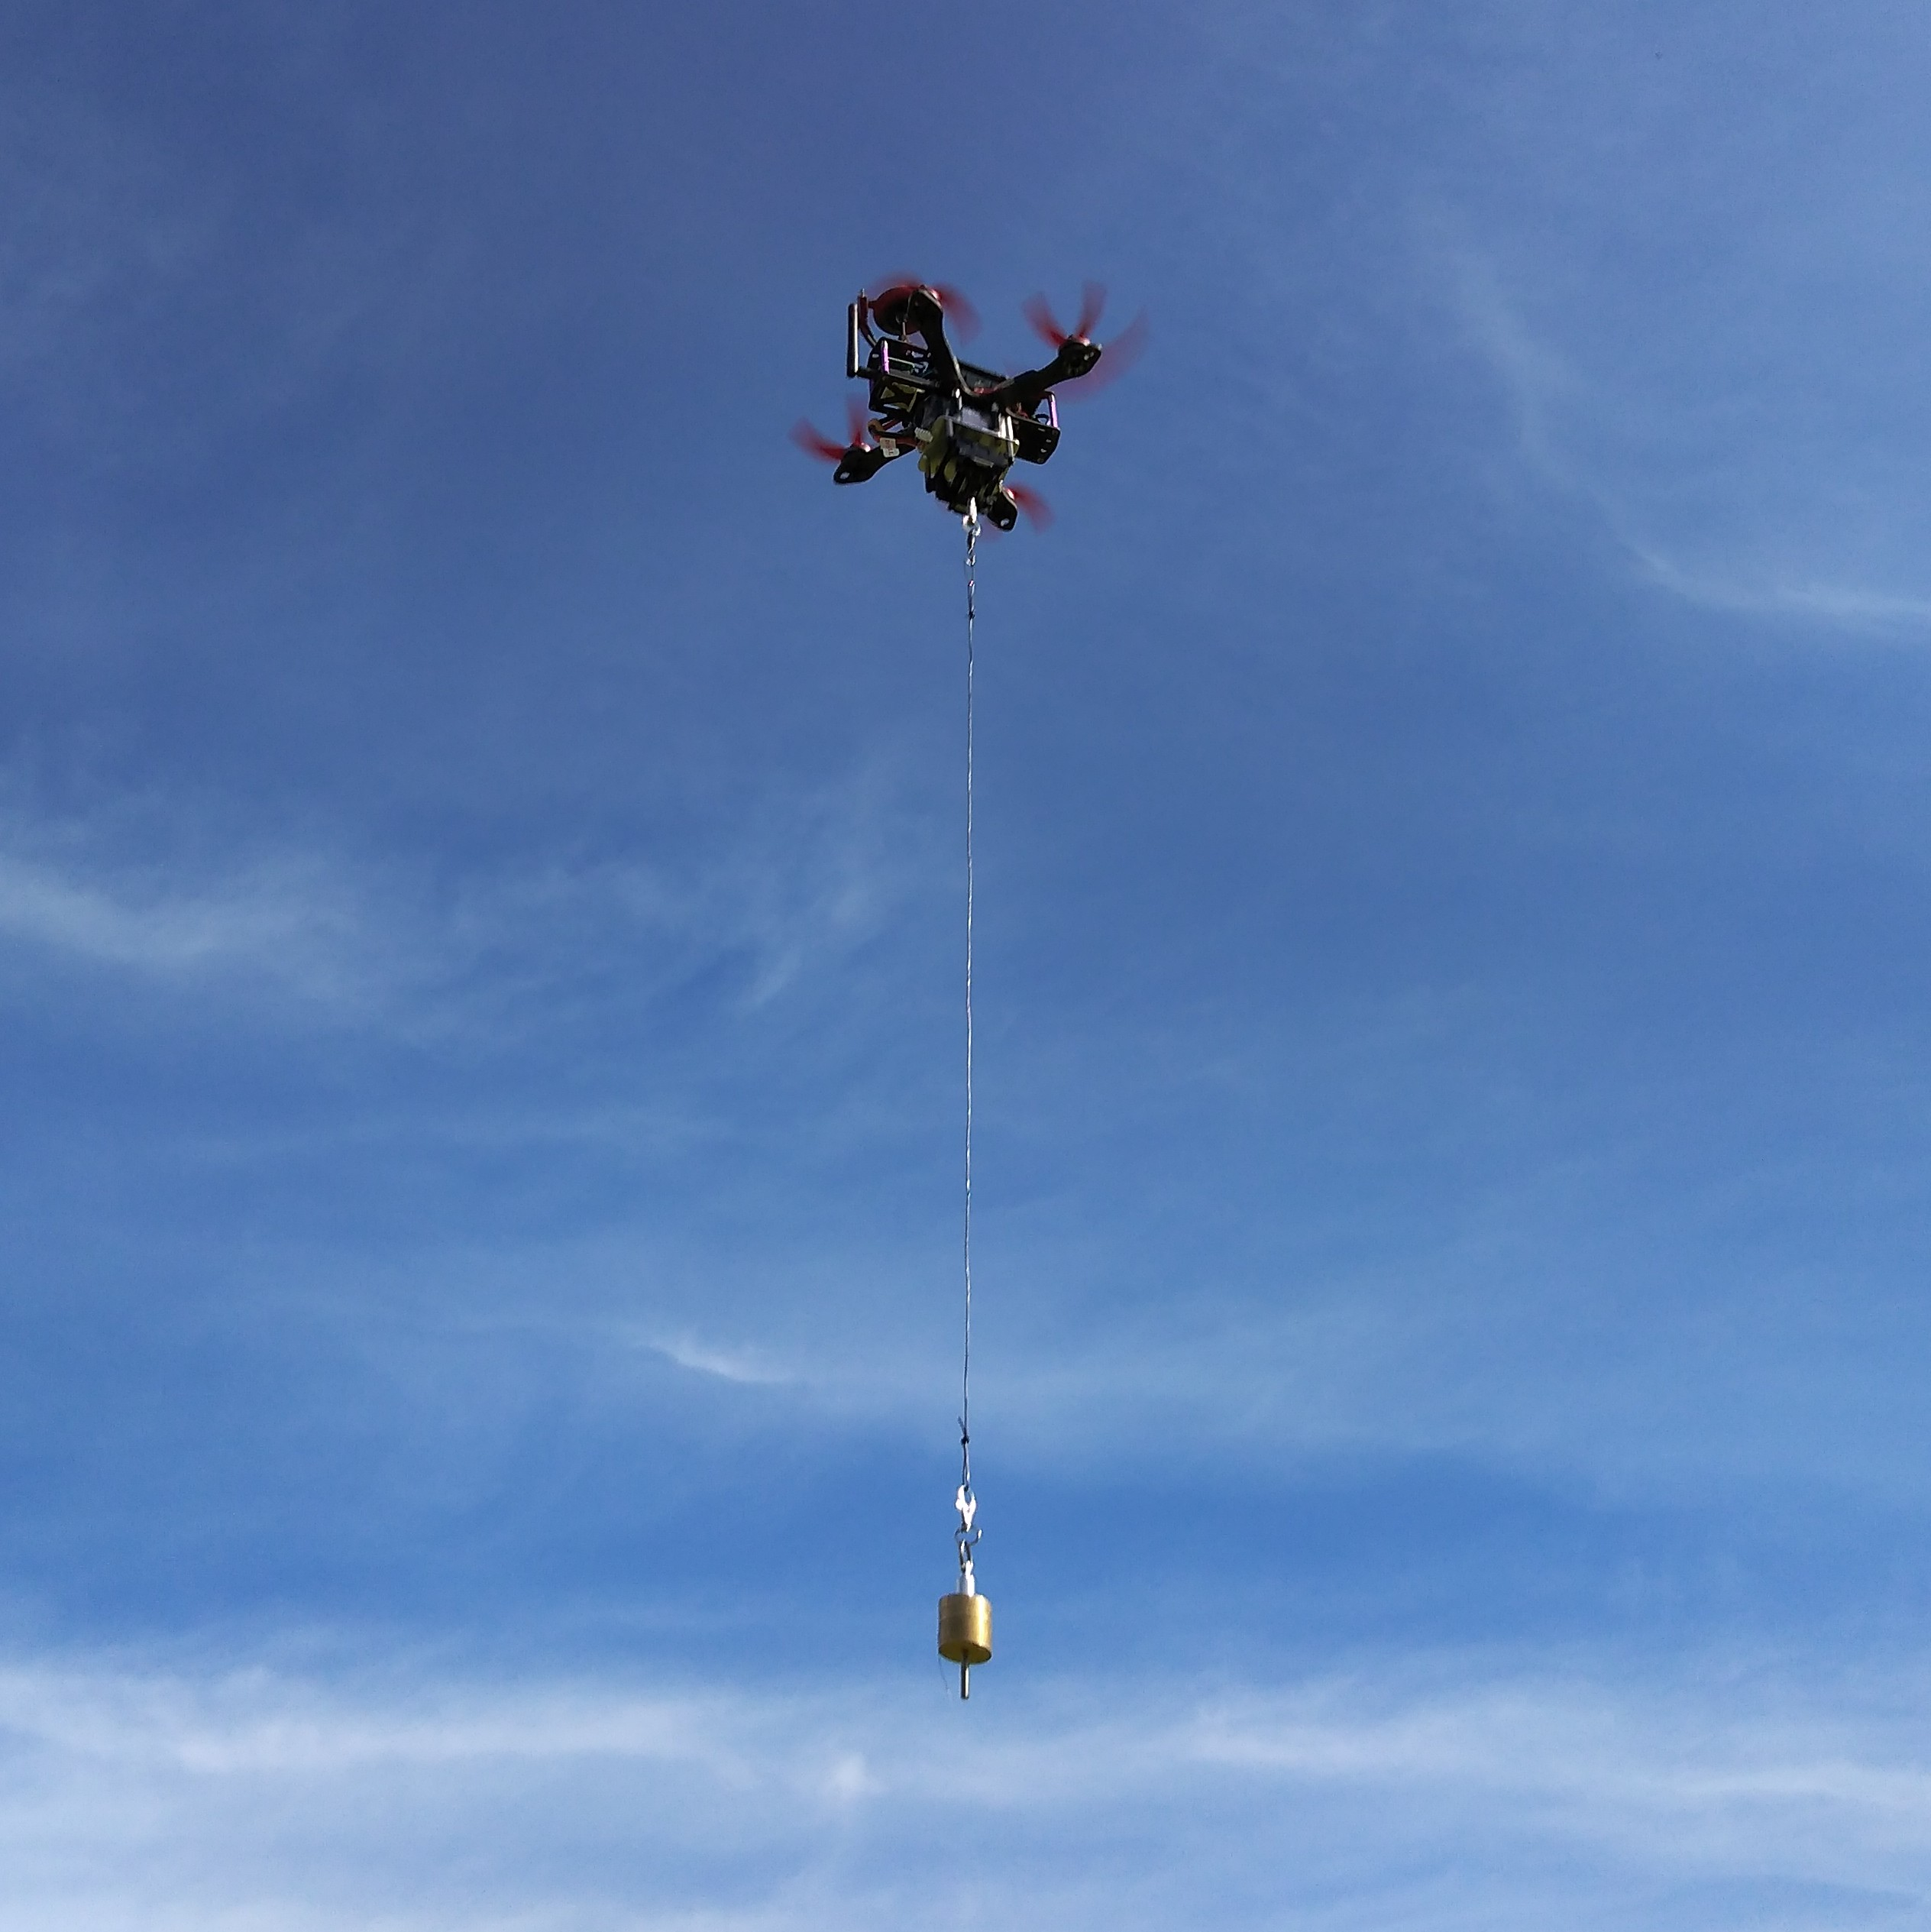
\includegraphics[width=0.5\linewidth]{honeybee_with_payload.jpg}
            \caption{Practical flight with Honeybee and a suspended payload}
            \label{fig:honeybee_with_payload}
        \end{figure}

        \paragraph
        Figure~\ref{fig:honeybee_with_payload} shows Honeybee in flight with a suspended payload.
        Numerous flights were performed with different 
        payload masses, 
        cable lengths, 
        wind conditions, 
        and even with a more complex elongated payload.
        The system identification methods were then performed on the data resulting from this range of different use cases.
        The major differences between the simulations and practical flights involve the attachment of the payload and wind disturbances.
        In simulation, the payload cable is attached to the exact \gls{CoM} of the mulitrotor.
        However, due to practical constraints, the cable is attached slightly below the \gls{CoM} of Honeybee.
        Practical flights are also influenced by wind disturbances, therefore this effect is also investigated in the sections below.
        In this chapter, wind conditions are referenced by the wind speed recorded by the website, www.yr.no, 
        for the hour of day of the flight.
        
        % \begin{itemize}
        %     \item Method for generating data
        %     \item Plot example of training data
        %     \item picture of practical flight single and double
        %     \item Discuss difference between \gls{SITL} and prac
        %     \begin{itemize}
        %         \item Noise 
        %         \item wind
        %         \item \gls{CoM}
        %     \end{itemize}
        %     \item plot hover of prac vs \gls{SITL} to show noise and disturbance
        % \end{itemize}

        % \paragraph
        % In Chapter~\ref{chap:system_id} it was noted that the optimal length of training data 
        % often only included 2 velocity steps responses.
        % This means the models were trained on a very small sample of step sizes 
        % and need to extrapolate the dynamics of other step sizes.
        
    \FloatBarrier\section{Parameter estimation with practical data}
        
        %% ?? Add this if there is time
        % \subsection{Mass estimation} 
        
        %     As discussed in Chapter~\ref{chap:system_id}, for this method to work, the mass of the mulitrotor needs to be known.
        %     If a heavier battery or an extra accessory is added to the vehicle, 
        %     the new vehicle mass will first have to be estimated in a separate flight, before the payload can be attached.
        %     This is one of the disadvantages of the white-box modelling with parameter estimation based techniques.
        %     The method is designed with a specific system in mind 
        %     and needs to be adjusted and redesigned for every deviation from the the pre-assumed configuration.
        %     In contrast, the data-driven technique is a general solution which works for a much wider range of system configurations.
        %     The data-driven technique is not readjusted for an added vehicle mass, 
        %     since the whole model is estimated instead of specific parameters.

        \FloatBarrier\subsection{Simple payload cable length estimation}
            
            \paragraph
            The \gls{PE} for the cable length estimation is calculated here as,
            \begin{equation}
                PE = \frac{ l_{actual} - l_{estimated} }{ l_{actual} } \times 100 \%,
            \end{equation}
            where $l_{actual}$ is the actual cable length and $l_{estimated}$ is the estimated cable length.
                
            \begin{figure}[htb]
    \centering
    \begin{tikzpicture}
        \begin{axis}[            
            xlabel = Length of training data,
            ylabel = Estimated cable length,
            x unit = \si{\second},
            y unit = \%,
            xmin = 0,   xmax = 15,
            ymin = -50,   ymax = 150,
            grid = major,
            legend cell align = left,
            legend pos = north east,
            grid style = dashed,
            legend style = {font = \scriptsize},
            label style = {font = \scriptsize},
            tick label style = {font = \scriptsize},
            width = 0.95\columnwidth,
            height = 0.5\columnwidth,
            % initialize Dark2
            cycle list/Dark2,
            % combine it with 'mark list*':
            cycle multiindex* list = {
                Dark2\nextlist
            }
        ]

        \addplot+[mark = none, style = solid, ultra thick] 
        table[x = train_time, y = percentage_error, col sep = comma] 
        {results/csv/cable_length_vs_train_time_Prac_2021-08-23_01_l-0.5_mp-0.2_wind-0.5.csv_10_0.5.csv};
        \addlegendentry{$m_p =$~\SI{0.2}{\kilo\gram}, $l =$~\SI{0.5}{\meter}}

        \addplot+[mark = none, style = solid, ultra thick] 
        table[x = train_time, y = percentage_error, col sep = comma] 
        {results/csv/cable_length_vs_train_time_Prac_2021-08-20_01_l-1_mp-0.1_wind-0.5.csv_10_1.csv};
        \addlegendentry{$m_p =$~\SI{0.1}{\kilo\gram}, $l =$~\SI{1}{\meter}}        

        \addplot+[mark = none, style = solid, ultra thick] 
        table[x = train_time, y = percentage_error, col sep = comma] 
        {results/csv/cable_length_vs_train_time_Prac_2021-08-20_02_l-2_mp-0.3-wind-0.5.csv_10_2.csv};
        \addlegendentry{$m_p =$~\SI{0.3}{\kilo\gram}, $l =$~\SI{2}{\meter}}

        \addplot+[mark = none, style = solid, ultra thick] 
        table[x = train_time, y = percentage_error, col sep = comma] 
        {results/csv/cable_length_vs_train_time_Prac_2021-08-20_03_l-1_mp-0.2_wind-0.5.csv_10_1.csv};
        \addlegendentry{$m_p =$~\SI{0.2}{\kilo\gram}, $l =$~\SI{1}{\meter}}
        
        \end{axis}
    \end{tikzpicture} 
    
    \caption{}
    \label{fig:cable_length_vs_train_time}
\end{figure}


            \begin{figure}[htb]
    \centering
    \begin{tikzpicture}
        \begin{axis}[            
            xlabel = Length of training data,
            ylabel = Percentage Error,
            x unit = \si{\second},
            y unit = \%,
            xmin = 0,       xmax = 12,
            ymin = -50,     ymax = 100,
            grid = major,
            legend cell align = left,
            legend pos = north east,
            grid style = dashed,
            legend style = {font = \scriptsize},
            label style = {font = \scriptsize},
            tick label style = {font = \scriptsize},
            width = 0.95\columnwidth,
            height = 0.5\columnwidth,
            % initialize Dark2
            cycle list/Dark2,
            % combine it with 'mark list*':
            cycle multiindex* list = {
                Dark2\nextlist
            }
        ]
        
        \addplot+[mark = none, style = solid, ultra thick] 
        table[x = train_time, y = percentage_error, col sep = comma] 
        {results/csv/cable_length_vs_train_time_Prac_2021-08-20_03_l-1_mp-0.2_wind-0.5.csv_10_1.csv};
        \addlegendentry{wind speed $\approx~$\SI{0.5}{\metre/\second}}

        \addplot+[mark = none, style = solid, ultra thick] 
        table[x = train_time, y = percentage_error, col sep = comma] 
        {results/csv/cable_length_vs_train_time_Prac_2021-08-12_03_manual_x_vel_steps_2mps.csv_10_1.csv};
        \addlegendentry{wind speed $\approx~$\SI{2}{\metre/\second}}

        \addplot+[mark = none, style = solid, ultra thick] 
        table[x = train_time, y = percentage_error, col sep = comma] 
        {results/csv/cable_length_vs_train_time_Prac_2021-08-12_02_manual_x_vel_steps_4mps.csv_20_1.csv};
        \addlegendentry{wind speed $\approx~$\SI{4}{\metre/\second}}

        \addplot+[mark = none, style = solid, ultra thick] 
        table[x = train_time, y = percentage_error, col sep = comma] 
        {results/csv/cable_length_vs_train_time_Prac_2021-08-26_01_l-1_mp-0.2_wind-6.csv_10_1.csv};
        \addlegendentry{wind speed $\approx~$\SI{6}{\metre/\second}}

        \end{axis}
    \end{tikzpicture} 
    
    \caption{Cable length estimation error as a function of length of training data with wind disturbances
        ($m_p =$~\SI{0.2}{\kilo\gram}, $l =$~\SI{1}{\meter}).}
    \label{fig:cable_length_vs_train_time_wind}
\end{figure}

        
        \FloatBarrier\subsection{Dynamic payload cable length estimation}

            \paragraph

            \begin{figure}[htb]
    \centering
    \begin{tikzpicture}
        \begin{axis}[            
            xlabel = Length of training data,
            ylabel = Estimated cable length,
            x unit = \si{\second},
            y unit = \si{\metre},
            xmin = 0,   xmax = 10,
            ymin = 0,   ymax = 4,
            grid = major,
            legend cell align = left,
            legend pos = north east,
            grid style = dashed,
            legend style = {font = \scriptsize},
            label style = {font = \scriptsize},
            tick label style = {font = \scriptsize},
            width = 0.95\columnwidth,
            height = 0.5\columnwidth,
            % initialize Dark2
            cycle list/Dark2,
            % combine it with 'mark list*':
            cycle multiindex* list = {
                Dark2\nextlist
            }
        ]

        \addplot+[mark = none, style = solid, ultra thick] 
        table[x = train_time, y = estimated_length, col sep = comma] 
        {results/csv/cable_length_vs_train_time_Prac_2021-08-23_04_double_pend_m1_0.2_m2_0.1_l1-0.5_l2_0.62_wind-0.5.csv_20_0.5.csv};
        
        \end{axis}
    \end{tikzpicture} 
    
    \caption{Estimated cable length as a function of length of training data for a dynamic payload
    ($m_1 =$~\SI{0.2}{\kilo\gram}, $l_1 =$~\SI{0.5}{\meter}, $m_2 =$~\SI{0.1}{\kilo\gram}, $l_2 =$~\SI{0.6}{\meter}) }
    \label{fig:double_pend_cable_length_vs_train_time}
\end{figure}

            
    \FloatBarrier\section{Data-driven system identification with practical data}

        \paragraph
        It was shown that the simulation environment 
        In Chapter~\ref{chap:system_id} it was shown that the data-driven methods 
        build accurate state prediction models for the considered system.
        It was also shown in Chapter~\ref{chap:modelling} that the simulation environment is a realistic representation of the practical system.
        However, there are still differences between simulations and practical flight.
        Therefore the data-driven algorithms are applied to practical flight data in this chapter 
        to investigate their performance in a practical implementation.

        \FloatBarrier\subsection{Length of training data}

            \paragraph
            As discussed in Section~\ref{sec:sys_id_length_of_data}, 
            the length of training data used in the model has a large effect on prediction accuracy.
            The length of training data required for accurate models is largely influenced by the amount of wind disturbance during flight.
            Figure~\ref{fig:wind_Ttrain} shows prediction error as a function of training data length for different wind conditions.
            Its clear that the prediction error decreases with increasing wind speeds.
            It appears that for wind speeds lower than \SI{2}{\metre/\second}, 
            the minimum prediction error is not significantly improved with decreasing wind speeds.
            This may be because the flight dynamics is not significantly affected at such low wind speeds.
            
            \paragraph
            Wind adds an unmeasured input, also referred to as process noise, to the plant and this is not accounted for in the model.
            As discussed in Section~\ref{sec:noise}, the constant offset is subtracted from the acceleration setpoint data, 
            which results in a signal with a zero mean.
            This accounts for the constant component in the acceleration setpoint signal required to counteract the mean force of the wind.
            However, the wind speed deviates randomly from the mean speed which results in random process noise in the plant.

            % \paragraph
            % It appears that for higher wind speeds, 
            % the prediction error does not reach a peak value within the considered range of training data lengths.
            
            % This is expected, since the algorithms require longer lengths of training data to  
            
            \begin{figure}[htb]
    \centering
    \begin{tikzpicture}
        \begin{axis}[            
            xlabel = Length of training data,
            ylabel = $\overline{NMAE}$ \phantom{~},
            x unit = \si{\second},
            y unit = \%,
            xmin = 5,     xmax = 120,
            ymin = 3.2,  ymax = 15,
            grid = major,
            legend cell align = left,
            legend pos = north east,
            grid style = dashed,
            legend style = {font = \scriptsize},
            label style = {font = \scriptsize},
            tick label style = {font = \scriptsize},
            width = 0.95\columnwidth,
            height = 0.5\columnwidth,
            % initialize Dark2
            cycle list/Dark2,
            % combine it with 'mark list*':
            cycle multiindex* list = {
                Dark2\nextlist
            }
        ]

        \addplot+[mark = none, style = solid, ultra thick] 
        table[x = T_train, y expr = {\thisrow{NMAE_mean}*100}, col sep = comma] 
        {results/csv/NMAE_vs_Ntrain_Prac_2021-08-20_03_l-1_mp-0.2_wind-0.5.csv_dmd_angle.csv};
        \addlegendentry{0.5 m/s winds}

        \addplot+[mark = none, style = solid, ultra thick] 
        table[x = T_train, y expr = {\thisrow{NMAE_mean}*100}, col sep = comma] 
        {results/csv/NMAE_vs_Ntrain_Prac_2021-08-12_03_manual_x_vel_steps_2mps.csv_dmd_angle.csv};
        \addlegendentry{2 m/s winds}

        \addplot+[mark = none, style = solid, ultra thick] 
        table[x = T_train, y expr = {\thisrow{NMAE_mean}*100}, col sep = comma] 
        {results/csv/NMAE_vs_Ntrain_Prac_2021-08-12_02_manual_x_vel_steps_4mps.csv_dmd_angle.csv};
        \addlegendentry{4 m/s winds}

        \addplot+[mark = none, style = solid, ultra thick] 
        table[x = T_train, y expr = {\thisrow{NMAE_mean}*100}, col sep = comma] 
        {results/csv/NMAE_vs_Ntrain_Prac_2021-08-26_01_l-1_mp-0.2_wind-6.csv_dmd_angle.csv};
        \addlegendentry{6 m/s winds}

        \end{axis}
    \end{tikzpicture} 
    
    \caption{Effect of wind on \gls{DMD} prediction errors for different lengths of practical training data
    ($m_p =$~\SI{0.2}{\kilo\gram}, $l =$~\SI{1}{\meter}, $T_s =$~\SI{0.03}{\second}).}
    \label{fig:wind_Ttrain}
\end{figure}

            
            \paragraph
            \gls{HAVOK} and \gls{DMD} perform similarly
            Figure~\ref{fig:havok_vs_dmd_Ttrain_2mps} shows the prediction error of \gls{DMD} and \gls{HAVOK} models
            
            \begin{figure}[htb]
    \centering
    \begin{tikzpicture}
        \begin{axis}[            
            xlabel = Length of training data,
            ylabel = $\overline{NMAE}$ \phantom{~},
            x unit = \si{\second},
            y unit = \%,
            xmin = 5,     xmax = 120,
            ymin = 3.2,  ymax = 15,
            grid = major,
            legend cell align = left,
            legend pos = north east,
            grid style = dashed,
            legend style = {font = \scriptsize},
            label style = {font = \scriptsize},
            tick label style = {font = \scriptsize},
            width = 0.95\columnwidth,
            height = 0.5\columnwidth,
            % initialize Dark2
            cycle list/Dark2,
            % combine it with 'mark list*':
            cycle multiindex* list = {
                Dark2\nextlist
            }
        ]

        \addplot+[mark = none, style = solid, ultra thick] 
        table[x = T_train, y expr = {\thisrow{NMAE_mean}*100}, col sep = comma] 
        {results/csv/NMAE_vs_Ntrain_Prac_2021-08-12_03_manual_x_vel_steps_2mps.csv_dmd_angle.csv};
        \addlegendentry{DMD}

        \addplot+[mark = none, style = solid, ultra thick] 
        table[x = T_train, y expr = {\thisrow{NMAE_mean}*100}, col sep = comma] 
        {results/csv/NMAE_vs_Ntrain_Prac_2021-08-12_03_manual_x_vel_steps_2mps.csv_havok_angle.csv};
        \addlegendentry{HAVOK}

        \end{axis}
    \end{tikzpicture} 
    
    \caption{\gls{DMD} and \gls{HAVOK} prediction errors for different lengths of practical training data
    ($m =$~\SI{0.206}{\kilo\gram}, $l =$~\SI{1}{\meter}, $T_s =$~\SI{0.03}{\second}).}
    \label{fig:havok_vs_dmd_Ttrain_2mps}
\end{figure}


            Also plot \gls{DMD} vs \gls{HAVOK} for high winds ??
            

            plot \gls{NMAE} vs Ttrain
            \begin{itemize}
                \item Plot strong wind vs less wind vs no wind
                \item \gls{HAVOK} vs \gls{DMD}
                \item Plot single pend vs double pend
            \end{itemize}
            
        \FloatBarrier\subsection{Hyperparameters}
            
            \paragraph
            As discussed in Section~\ref{sec:hyperparameters}, 
            the prediction error generally improves with an increasing number of delay-coordinates 
            because the number of parameters in the model increases.
            However, the prediction error reaches a pareto optimum, 
            after which the error does not significantly decrease with an increasing number of terms anymore.
            Figure~\ref{fig:havok_vs_dmd_q_2mps} shows the prediction error as a function of the number of delay-coordinates
            for practical flight data.
            Even though the pareto elbow is not as smooth and clear as models build from simulation data, 
            the elbow can still be identified.            
            % Note that the pareto elbow is not as smooth and clear as shown in Section~\ref{sec:hyperparameters}.
            % This may due to random 
            % The pareto optimal models for practical data have significantly more delay-coordinates than

            \begin{figure}[htb]
    \centering
    \begin{tikzpicture}
        \begin{axis}[            
            xlabel = {Number of delay-coordinates, $q$},
            ylabel = $\overline{NMAE}$ \phantom{~},
            % x unit = \si{\second},
            y unit = \%,
            xmin = 5,     xmax = 90,
            ymin = 3.5,  ymax = 7.5,
            grid = major,
            legend cell align = left,
            legend pos = north east,
            grid style = dashed,
            legend style = {font = \scriptsize},
            label style = {font = \scriptsize},
            tick label style = {font = \scriptsize},
            width = 0.95\columnwidth,
            height = 0.5\columnwidth,
            % initialize Dark2
            cycle list/Dark2,
            % combine it with 'mark list*':
            cycle multiindex* list = {
                Dark2\nextlist
            }
        ]

        \addplot+[mark = none, style = solid, ultra thick] 
        table[x = q, y expr = {\thisrow{NMAE_mean}*100}, col sep = comma] 
        {results/csv/NMAE_vs_q_Prac_2021-08-12_03_manual_x_vel_steps_2mps_q.csv_dmd_angle.csv};
        \addlegendentry{DMD}

        \addplot+[mark = none, style = solid, ultra thick] 
        table[x = q, y expr = {\thisrow{NMAE_mean}*100}, col sep = comma] 
        {results/csv/NMAE_vs_q_Prac_2021-08-12_03_manual_x_vel_steps_2mps_q.csv_havok_angle.csv};
        \addlegendentry{HAVOK}

        % \addplot+[mark = none, style = solid, ultra thick] 
        % table[x = q, y expr = {\thisrow{NMAE_mean}*100}, col sep = comma] 
        % {results/csv/NMAE_vs_q_Prac_2021-08-20_03_l-1_mp-0.2_wind-0.5_q.csv_dmd_angle.csv};
        % \addlegendentry{DMD}

        % \addplot+[mark = none, style = solid, ultra thick] 
        % table[x = q, y expr = {\thisrow{NMAE_mean}*100}, col sep = comma] 
        % {results/csv/NMAE_vs_q_Prac_2021-08-20_03_l-1_mp-0.2_wind-0.5_q.csv_havok_angle.csv};
        % \addlegendentry{HAVOK}


        \end{axis}
    \end{tikzpicture} 
    
    \caption{\gls{DMD} and \gls{HAVOK} prediction errors for different number of delays included in the model
    ($m =$~\SI{0.206}{\kilo\gram}, $l =$~\SI{1}{\meter}, $T_s =$~\SI{0.03}{\second}, wind speed $\approx~$\SI{2}{\metre/\second}).}
    \label{fig:havok_vs_dmd_q_2mps}
\end{figure}


            % \begin{figure}[htb]
    \centering
    \begin{tikzpicture}
        \begin{semilogyaxis}[            
            xlabel = Index of mode,
            ylabel = Singular value,
            % x unit = \si{\second},
            % y unit = \si{\second},
            xmin = 0,     xmax = 183,
            ymin = 1e-5,  ymax = 1e4,
            grid = major,
            legend cell align = left,
            legend pos = north east,
            grid style = dashed,
            legend style = {font = \scriptsize},
            label style = {font = \scriptsize},
            tick label style = {font = \scriptsize},
            width = 0.95\columnwidth,
            height = 0.5\columnwidth,
            % initialize Dark2
            cycle list/Dark2,
            % combine it with 'mark list*':
            cycle multiindex* list = {
                Dark2\nextlist
            }
        ]

        \addplot+[only marks, mark = *, ultra thin, mark options={scale=0.7}] 
        table[x = index, y = S, col sep = comma] 
        {results/csv/Singular_values_Prac_2021-08-12_03_manual_x_vel_steps_2mps_q.csv_havok_angle_Ttrain_50_q91_p52.csv};
        \addlegendentry{Significant modes}

        \addplot+[only marks, mark = *, ultra thin, mark options={scale=0.7}] 
        table[x = index, y = S, col sep = comma] 
        {results/csv/Singular_values_Prac_2021-08-12_03_manual_x_vel_steps_2mps_q.csv_havok_angle_Ttrain_50_q91_p52_trunc.csv};
        \addlegendentry{Truncated modes}

        \end{semilogyaxis}
    \end{tikzpicture} 
    
    \caption{Significant and truncated singular values of a \gls{HAVOK} model produced from practical data
    ($m_p =$~\SI{0.2}{\kilo\gram}, $l =$~\SI{0.5}{\meter}, $T_s =$~\SI{0.03}{\second}, $T_{train} =$~\SI{60}{\second}.)}
    \label{fig:prac_singular_values}
\end{figure}

            % Difference between SITl and practical (same input steps)
            % This is due to wind disturbance
            % Plot wind vs less wind vs no wind
            
        \FloatBarrier\subsection{System parameters}

            \paragraph
            It was shown with multiple simulations in Section~\ref{sec:system_params} 
            that the system identification methods work for a range of different payload parameters.
            Figure~\ref{fig:prac_system_params} shows the prediction error for different payloads with practical data.
            This shows that the proposed methods also work in practice with different payloads.
            The `double-descent' trend is clearly seen in all of the plots, 
            where the prediction error increases slightly after a specific length of training data,            
            
            \begin{figure}[htb]
    \centering
    \begin{tikzpicture}
        \begin{axis}[            
            xlabel = Length of training data,
            ylabel = $\overline{NMAE}$ \phantom{~},
            x unit = \si{\second},
            y unit = \%,
            xmin = 5,     xmax = 120,
            ymin = 2.8,  ymax = 7.8,
            grid = major,
            legend cell align = left,
            legend pos = north east,
            grid style = dashed,
            legend style = {font = \scriptsize},
            label style = {font = \scriptsize},
            tick label style = {font = \scriptsize},
            width = 0.95\columnwidth,
            height = 0.5\columnwidth,
            % initialize Dark2
            cycle list/Dark2,
            % combine it with 'mark list*':
            cycle multiindex* list = {
                Dark2\nextlist
            }
        ]
         
        \addplot+[mark = none, style = solid, ultra thick] 
        table[x = T_train, y expr = {\thisrow{NMAE_mean}*100}, col sep = comma] 
        {results/csv/NMAE_vs_Ntrain_Prac_2021-08-20_01_l-1_mp-0.1_wind-0.5.csv_dmd_angle.csv};
        \addlegendentry{$m =$~\SI{0.1}{\kilo\gram}, $l = $~\SI{1}{\metre}}
        
        \addplot+[mark = none, style = solid, ultra thick] 
        table[x = T_train, y expr = {\thisrow{NMAE_mean}*100}, col sep = comma] 
        {results/csv/NMAE_vs_Ntrain_Prac_2021-08-20_02_l-2_mp-0.3-wind-0.5.csv_dmd_angle.csv};
        \addlegendentry{$m =$~\SI{0.3}{\kilo\gram}, $l = $~\SI{2}{\metre}}
        
        \addplot+[mark = none, style = solid, ultra thick] 
        table[x = T_train, y expr = {\thisrow{NMAE_mean}*100}, col sep = comma] 
        {results/csv/NMAE_vs_Ntrain_Prac_2021-08-20_03_l-1_mp-0.2_wind-0.5.csv_dmd_angle.csv};
        \addlegendentry{$m =$~\SI{0.2}{\kilo\gram}, $l = $~\SI{1}{\metre}}
        
        \end{axis}
    \end{tikzpicture} 

    \caption{DMD prediction error as a function of training data length for different payload parameters}
    \label{fig:prac_system_params}
\end{figure}


        \FloatBarrier\subsection{Predictions}

            \paragraph
            Notice how the prediction deviates more from the measured value as time progresses.
            This is because of the build up, discrete, initial condition 

            \begin{figure}[htb]
    \centering
    \begin{tikzpicture}
        \begin{axis}[            
            xlabel = Time,
            ylabel = Payload angle,
            x unit = \si{\second},
            y unit = \si{\degree},
            xmin = 0,   xmax = 20,
            ymin = -20,  ymax = 25,
            grid = major,
            legend cell align = left,
            legend pos = north east,
            grid style = dashed,
            legend style = {font = \scriptsize},
            label style = {font = \scriptsize},
            tick label style = {font = \scriptsize},
            width = 0.95\columnwidth,
            height = 0.5\columnwidth,
            % initialize Dark2
            cycle list/Dark2,
            % combine it with 'mark list*':
            cycle multiindex* list = {
                Dark2\nextlist
            }
        ]
        
        \addplot+[mark = none, style = solid, ultra thick] 
        table[x = time, y = theta, col sep = comma] 
        {results/csv/step_predictions_Prac_2021-08-20_02_l-2_mp-0.3-wind-0.5.csv_dmd_737.csv};
        \addlegendentry{Measured}

        \addplot+[mark = none, style = dashed, ultra thick] 
        table[x = time, y = theta_hat, col sep = comma] 
        {results/csv/step_predictions_Prac_2021-08-20_02_l-2_mp-0.3-wind-0.5.csv_dmd_737.csv};
        \addlegendentry{DMD prediction}

        \end{axis}
    \end{tikzpicture} 
    
    \caption{Model predictions of practical flight data with an suspended payload for a North velocity step input
        ($l =$~\SI{2}{\meter}, $m_p =$~\SI{0.3}{\kilo\gram})}
    \label{fig:prac_pediction_single_pend_theta_black}
\end{figure}


            \paragraph
            
            \begin{figure}[htb]
    \centering
    \begin{tikzpicture}
        \begin{axis}[            
            xlabel = Time,
            ylabel = North velocity,
            x unit = \si{\second},
            y unit = \si{\metre/\second},
            xmin = 0,   xmax = 20,
            ymin = -2,  ymax = 1.5,
            grid = major,
            legend cell align = left,
            legend pos = north east,
            grid style = dashed,
            legend style = {font = \scriptsize},
            label style = {font = \scriptsize},
            tick label style = {font = \scriptsize},
            width = 0.95\columnwidth,
            height = 0.5\columnwidth,
            % initialize Dark2
            cycle list/Dark2,
            % combine it with 'mark list*':
            cycle multiindex* list = {
                Dark2\nextlist
            }
        ]
        
        \addplot+[mark = none, style = solid, ultra thick] 
        table[x = time, y = vel, col sep = comma] 
        {results/csv/step_predictions_Prac_2021-08-20_02_l-2_mp-0.3-wind-0.5.csv_dmd_737.csv};
        \addlegendentry{Measured}

        \addplot+[mark = none, style = dashed, ultra thick] 
        table[x = time, y = vel_hat, col sep = comma] 
        {results/csv/step_predictions_Prac_2021-08-20_02_l-2_mp-0.3-wind-0.5.csv_dmd_737.csv};
        \addlegendentry{DMDc prediction}

        \end{axis}
    \end{tikzpicture} 
    
    \caption{Model predictions of practical flight data with a suspended payload for a North velocity step input
        ($l =$~\SI{2}{\meter}, $m_p =$~\SI{0.3}{\kilo\gram}, wind speed $\approx~$\SI{0.5}{\metre/\second}).}
    \label{fig:prac_pediction_single_pend_vel_black}
\end{figure}

        
        \FloatBarrier\subsection{Extended dimensions}

            \paragraph
            This method can easily be extended to damp the swing angle in both the $x$ and $y$ directions.
            Show new control vector and new state vector.
            Talk about steps given.
            Figure~\ref{fig:xy_predictions} \gls{DMD} predictions

            \begin{figure}
                \captionsetup[subfigure]{justification=centering}
                \centering
                \begin{subfigure}{\columnwidth}
    \centering
    \begin{tikzpicture}
        \begin{axis}[            
            xlabel = Time,
            ylabel = North axis payload angle,
            x unit = \si{\second},
            y unit = \si{\degree},
            xmin = 0,   xmax = 20,
            ymin = -20,  ymax = 20,
            grid = major,
            legend cell align = left,
            legend pos = north east,
            grid style = dashed,
            legend style = {font = \scriptsize},
            label style = {font = \scriptsize},
            tick label style = {font = \scriptsize},
            width = 0.95\columnwidth,
            height = 0.3\columnwidth,
            % initialize Dark2
            cycle list/Dark2,
            % combine it with 'mark list*':
            cycle multiindex* list = {
                Dark2\nextlist
            }
        ]
        
        \addplot+[mark = none, style = solid, ultra thick] 
        table[x = time, y = theta_x, col sep = comma] 
        {results/csv/step_predictions_Prac_2021-08-23_02_l-0.5_mp-0.2_wind-0.5_XY_steps.csv_dmd_746.csv};
        \addlegendentry{Measured}

        \addplot+[mark = none, style = dashed, ultra thick] 
        table[x = time, y = theta_x_hat, col sep = comma] 
        {results/csv/step_predictions_Prac_2021-08-23_02_l-0.5_mp-0.2_wind-0.5_XY_steps.csv_dmd_746.csv};
        \addlegendentry{DMD prediction}

        \end{axis}
    \end{tikzpicture} 

\end{subfigure}
 % subfigure
                \begin{figure}[htb]
    \centering
    \begin{tikzpicture}
        \begin{axis}[            
            xlabel = Time,
            ylabel = Payload angle,
            x unit = \si{\second},
            y unit = \si{\degree},
            xmin = 0,   xmax = 20,
            ymin = -20,  ymax = 25,
            grid = major,
            legend cell align = left,
            legend pos = north east,
            grid style = dashed,
            legend style = {font = \scriptsize},
            label style = {font = \scriptsize},
            tick label style = {font = \scriptsize},
            width = 0.95\columnwidth,
            height = 0.5\columnwidth,
            % initialize Dark2
            cycle list/Dark2,
            % combine it with 'mark list*':
            cycle multiindex* list = {
                Dark2\nextlist
            }
        ]
        
        \addplot+[mark = none, style = solid, ultra thick] 
        table[x = time, y = theta_y, col sep = comma] 
        {results/csv/step_predictions_Prac_2021-08-23_02_l-0.5_mp-0.2_wind-0.5_XY_steps.csv_dmd_746.csv};
        \addlegendentry{Measured}

        \addplot+[mark = none, style = solid, ultra thick] 
        table[x = time, y = theta_y_hat, col sep = comma] 
        {results/csv/step_predictions_Prac_2021-08-23_02_l-0.5_mp-0.2_wind-0.5_XY_steps.csv_dmd_746.csv};
        \addlegendentry{DMD prediction}

        \end{axis}
    \end{tikzpicture} 
    
    \caption{Practical flight data and model predictions for the North and East directions
        ($m_p =$~\SI{0.2}{\kilo\gram}, $l =$~\SI{0.5}{\meter})}
    \label{fig:prac_pediction_xy_theta_y}
\end{figure}
 % subfigure
                \begin{figure}[htb]
    \centering
    \begin{tikzpicture}
        \begin{axis}[            
            xlabel = Time,
            ylabel = North velocity,
            x unit = \si{\second},
            y unit = \si{\metre/\second},
            xmin = 0,   xmax = 20,
            ymin = -2.5,  ymax = 2.5,
            grid = major,
            legend cell align = left,
            legend pos = north east,
            grid style = dashed,
            legend style = {font = \scriptsize},
            label style = {font = \scriptsize},
            tick label style = {font = \scriptsize},
            width = 0.95\columnwidth,
            height = 0.5\columnwidth,
            % initialize Dark2
            cycle list/Dark2,
            % combine it with 'mark list*':
            cycle multiindex* list = {
                Dark2\nextlist
            }
        ]
        
        \addplot+[mark = none, style = solid, ultra thick] 
        table[x = time, y = vel_x, col sep = comma] 
        {results/csv/step_predictions_Prac_2021-08-23_02_l-0.5_mp-0.2_wind-0.5_XY_steps.csv_dmd_746.csv};
        \addlegendentry{Measured}

        \addplot+[mark = none, style = solid, ultra thick] 
        table[x = time, y = vel_x_hat, col sep = comma] 
        {results/csv/step_predictions_Prac_2021-08-23_02_l-0.5_mp-0.2_wind-0.5_XY_steps.csv_dmd_746.csv};
        \addlegendentry{DMD prediction}

        \end{axis}
    \end{tikzpicture} 
    
    \caption{Practical flight data and model predictions for the North and East directions
        ($m_p =$~\SI{0.2}{\kilo\gram}, $l =$~\SI{0.5}{\meter})}
    \label{fig:prac_pediction_xy_vel_x}
\end{figure}
 % subfigure
                \begin{figure}[htb]
    \centering
    \begin{tikzpicture}
        \begin{axis}[            
            xlabel = Time,
            ylabel = North velocity,
            x unit = \si{\second},
            y unit = \si{\metre/\second},
            xmin = 0,   xmax = 20,
            ymin = -2.5,  ymax = 2.5,
            grid = major,
            legend cell align = left,
            legend pos = north east,
            grid style = dashed,
            legend style = {font = \scriptsize},
            label style = {font = \scriptsize},
            tick label style = {font = \scriptsize},
            width = 0.95\columnwidth,
            height = 0.5\columnwidth,
            % initialize Dark2
            cycle list/Dark2,
            % combine it with 'mark list*':
            cycle multiindex* list = {
                Dark2\nextlist
            }
        ]
        
        \addplot+[mark = none, style = solid, ultra thick] 
        table[x = time, y = vel_y, col sep = comma] 
        {results/csv/step_predictions_Prac_2021-08-23_02_l-0.5_mp-0.2_wind-0.5_XY_steps.csv_dmd_746.csv};
        \addlegendentry{Measured}

        \addplot+[mark = none, style = solid, ultra thick] 
        table[x = time, y = vel_y_hat, col sep = comma] 
        {results/csv/step_predictions_Prac_2021-08-23_02_l-0.5_mp-0.2_wind-0.5_XY_steps.csv_dmd_746.csv};
        \addlegendentry{DMD prediction}

        \end{axis}
    \end{tikzpicture} 
    
    \caption{Practical flight data and model predictions for the North and East directions
        ($m_p =$~\SI{0.2}{\kilo\gram}, $l =$~\SI{0.5}{\meter})}
    \label{fig:prac_pediction_xy_vel_y}
\end{figure}
 % subfigure
                \caption{Data-driven predictions of practical data for a model with both North and East axis dynamics}
                \label{fig:xy_predictions}  
            \end{figure}

        %     Maybe add plot error vs q if there is time??

        \FloatBarrier\subsection{Dynamic payload} 

            \paragraph
            As mentioned in Chapter~\ref{chap:system_id}, 
            one of the disadvantages of the white-box system identification approach
            is that it relies heavily on a priori modeling assumptions.
            When a payload is attached that deviates from the white-box modelling assumptions, 
            the performance of the system identification method decreases.
            However, the performance of the data-driven methods can handle this deviation
            because it does not rely on these assumptions.

            \paragraph
            One of the main assumptions of the white-box model considered in Section~\ref{sec:param_estimation},
            is that the suspended payload is a point mass.
            This reduced the considered suspended payload system to a simple pendulum.
            Figure~\ref{fig:practical_double_pendulum} shows a practical dynamic payload 
            which deviates significantly from this assumption.
            It shows a photo of an elongated payload 
            suspended from Honeybee during a practical flight.
            The mass distribution causes a relative rotation of the payload with respect to the suspended cable,
            which significantly affects the flight dynamics.

            \begin{figure}[!htb]
                \centering
                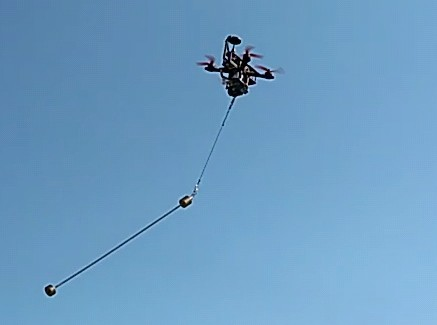
\includegraphics[width=0.6\linewidth]{practical_double_pendulum_2.jpg}
                \caption{Practical flight with an suspended elongated payload attached to Honeybee}
                \label{fig:practical_double_pendulum}
            \end{figure}

            \paragraph
            Theta prediction.

            \begin{figure}[htb]
    \centering
    \begin{tikzpicture}
        \begin{axis}[            
            xlabel = Time,
            ylabel = Payload angle,
            x unit = \si{\second},
            y unit = \si{\degree},
            xmin = 0,   xmax = 20,
            ymin = -20,  ymax = 25,
            grid = major,
            legend cell align = left,
            legend pos = north east,
            grid style = dashed,
            legend style = {font = \scriptsize},
            label style = {font = \scriptsize},
            tick label style = {font = \scriptsize},
            width = 0.95\columnwidth,
            height = 0.5\columnwidth,
            % initialize Dark2
            cycle list/Dark2,
            % combine it with 'mark list*':
            cycle multiindex* list = {
                Dark2\nextlist
            }
        ]
        
        \addplot+[mark = none, style = solid, ultra thick] 
        table[x = time, y = theta, col sep = comma] 
        {results/csv/step_predictions_Prac_2021-08-23_04_double_pend_m1_0.2_m2_0.1_l1-0.5_l2_0.62_wind-0.5.csv_dmd_201.csv};
        \addlegendentry{Measured}

        \addplot+[mark = none, style = dashed, ultra thick] 
        table[x = time, y = theta_hat, col sep = comma] 
        {results/csv/step_predictions_Prac_2021-08-23_04_double_pend_m1_0.2_m2_0.1_l1-0.5_l2_0.62_wind-0.5.csv_dmd_201.csv};
        \addlegendentry{DMD prediction}

        % \addplot+[mark = none, style = solid, ultra thick] 
        % table[x = time, y = theta, col sep = comma] 
        % {results/csv/step_predictions_Prac_2021-08-23_04_double_pend_m1_0.2_m2_0.1_l1-0.5_l2_0.62_wind-0.5.csv_dmd_201.csv};
        % \addlegendentry{White-box model}

        \end{axis}
    \end{tikzpicture} 
    
    \caption{Data-driven $\theta$ predictions of a double pendulum for a North velocity step input
        ($m_1 =$~\SI{0.2}{\kilo\gram}, $l_1 =$~\SI{0.5}{\meter}, $m_2 =$~\SI{0.1}{\kilo\gram}, $l_2 =$~\SI{0.6}{\meter})}
    \label{fig:prac_pediction_double_pend_theta_black}
\end{figure}

            
            \paragraph
            Vel prediction.
            Note that the prediction is propagated from an initial condition and the given input data only.
            The model does not use state measurements to readjust after the initial condition is taken.
            Because the model prediction matches the practical testing data so closely,
            it is expected that this model can effectively be used for a practical \gls{MPC} implementation. 

            % As discussed in Chapter~\ref{chap:control_systems}, 
            % this prediction model can be used in an \gls{MPC} to optimise the control input to actively damp the payload swing angles.
            % It was also noted in Chapter~\ref{chap:control_systems} that the accuracy of the model 
            % has a direct impact on the performance of the controller.
            % Because the model prediction matches the practical testing data so closely,
            % it is expected that this model will 

            \begin{figure}[htb]
    \centering
    \begin{tikzpicture}
        \begin{axis}[            
            xlabel = Time,
            ylabel = Payload angle,
            x unit = \si{\second},
            y unit = \si{\degree},
            xmin = 0,   xmax = 20,
            ymin = -2.5,  ymax = 2.5,
            grid = major,
            legend cell align = left,
            legend pos = north east,
            grid style = dashed,
            legend style = {font = \scriptsize},
            label style = {font = \scriptsize},
            tick label style = {font = \scriptsize},
            width = 0.95\columnwidth,
            height = 0.5\columnwidth,
            % initialize Dark2
            cycle list/Dark2,
            % combine it with 'mark list*':
            cycle multiindex* list = {
                Dark2\nextlist
            }
        ]
        
        \addplot+[mark = none, style = solid, ultra thick] 
        table[x = time, y = vel, col sep = comma] 
        {results/csv/step_predictions_Prac_2021-08-23_04_double_pend_m1_0.2_m2_0.1_l1-0.5_l2_0.62_wind-0.5.csv_dmd_201.csv};
        \addlegendentry{Measured}

        \addplot+[mark = none, style = dashed, ultra thick] 
        table[x = time, y = vel_hat, col sep = comma] 
        {results/csv/step_predictions_Prac_2021-08-23_04_double_pend_m1_0.2_m2_0.1_l1-0.5_l2_0.62_wind-0.5.csv_dmd_201.csv};
        \addlegendentry{DMD prediction}

        % \addplot+[mark = none, style = solid, ultra thick] 
        % table[x = time, y = theta, col sep = comma] 
        % {results/csv/step_predictions_Prac_2021-08-23_04_double_pend_m1_0.2_m2_0.1_l1-0.5_l2_0.62_wind-0.5.csv_dmd_201.csv};
        % \addlegendentry{White-box model}

        \end{axis}
    \end{tikzpicture} 
    
    \caption{Data-driven $V_N$ model predictions of a double pendulum for a North velocity step input
        ($m_1 =$~\SI{0.2}{\kilo\gram}, $l_1 =$~\SI{0.5}{\meter}, $m_2 =$~\SI{0.1}{\kilo\gram}, $l_2 =$~\SI{0.6}{\meter})}
    \label{fig:prac_pediction_double_pend_theta_black}
\end{figure}

            
            \paragraph
            Double pendulum: 
            \begin{itemize}
                \item Plot theta
                \item Plot velocity
                \item Plot theta prediction of white-box model
            \end{itemize}
            
        % \FloatBarrier\subsection{Extended dimensions}
        %     \begin{itemize}
        %         \item plot error vs T-train for XY
        %         \item plot predictions
        %         \item plot error vs T-train for XYZ
        %     \end{itemize}
        %     Maybe add this is there is time??
            
    \FloatBarrier\section{Swing damping control systems}

        \paragraph
        After the system identification phase, active swing damping control can be applied
        to the mulitrotor and payload system.
        The control architectures are summarised in Table~\ref{tbl:controller_summary} 
        by pairing the system identification techniques along with the appropriate controllers.
        It was firstly shown in Chapter~\ref{chap:system_id} that the system identifcation techniques worked in simulation.
        Emphasise that control is now applied in full \gls{SITL} simulation.

        \paragraph
        MATLAB is used to generate a \gls{MPC} \gls{ROS} node 
        This \gls{ROS} node receives state feedback from the Gazebo simulator,
        computes the optimal control action,
        and send the setpoint to PX4 through the package 'mavros'.

        \begin{table}[!h]
            \renewcommand{\arraystretch}{1.1}
            \centering
            \caption{Summary of the system identification techniques paired with the active damping controllers.}
            \begin{tabularx}{0.75\linewidth}{@{}lll@{}}
                \toprule
                \multicolumn{2}{c}{\textbf{System identification}}   & \textbf{Controller} \\
                \cmidrule(lr){1-2}
                Category    & Algorithm                     & \\
                \midrule
                White-box   & RLS mass estimator, and       & LQR \\
                            & FFT cable length estimator    & \\
                Black-box   & DMDc, or                      & MPC \\
                            & HAVOK                         & \\
                \bottomrule
            \end{tabularx}
            \label{tbl:controller_summary}
        \end{table}
        

        \FloatBarrier\subsection{Single pendulum}

            \begin{itemize}
                \item subplot prediction of data driven model. subplot prediction of white-box model
                \item plot \gls{MPC} vs \gls{LQR} v \gls{PID} (no wind) step = 1 m/s
                \item plot \gls{MPC} vs \gls{LQR} v \gls{PID} (no wind) step = 2 m/s
                \item plot \gls{DMDc} vs \gls{HAVOK} (\gls{DMD} - Havok)
                \item plot with wind disturbacne control
            \end{itemize}

        \FloatBarrier\subsection{Double pendulum}

            \begin{itemize}
                \item subplot prediction of data driven model. subplot prediction of white-box model
                \item plot \gls{MPC} vs \gls{LQR} v \gls{PID} (no wind)
                \item plot \gls{DMDc} vs \gls{HAVOK} (\gls{DMD} - Havok)
            \end{itemize}

    \section{HITL}

    \section{Conclusion}


